\hypertarget{phonefirewall__administration_8c}{
\section{/home/obale/sourcecode/myprograms/phone-firewall/src/phonefirewall\_\-administration.c File Reference}
\label{phonefirewall__administration_8c}\index{/home/obale/sourcecode/myprograms/phone-firewall/src/phonefirewall\_\-administration.c@{/home/obale/sourcecode/myprograms/phone-firewall/src/phonefirewall\_\-administration.c}}
}
{\tt \#include $<$stdio.h$>$}\par
{\tt \#include $<$stdlib.h$>$}\par
{\tt \#include $<$errno.h$>$}\par
{\tt \#include $<$string.h$>$}\par
{\tt \#include \char`\"{}libphonefirewall.h\char`\"{}}\par


Include dependency graph for phonefirewall\_\-administration.c:\nopagebreak
\begin{figure}[H]
\begin{center}
\leavevmode
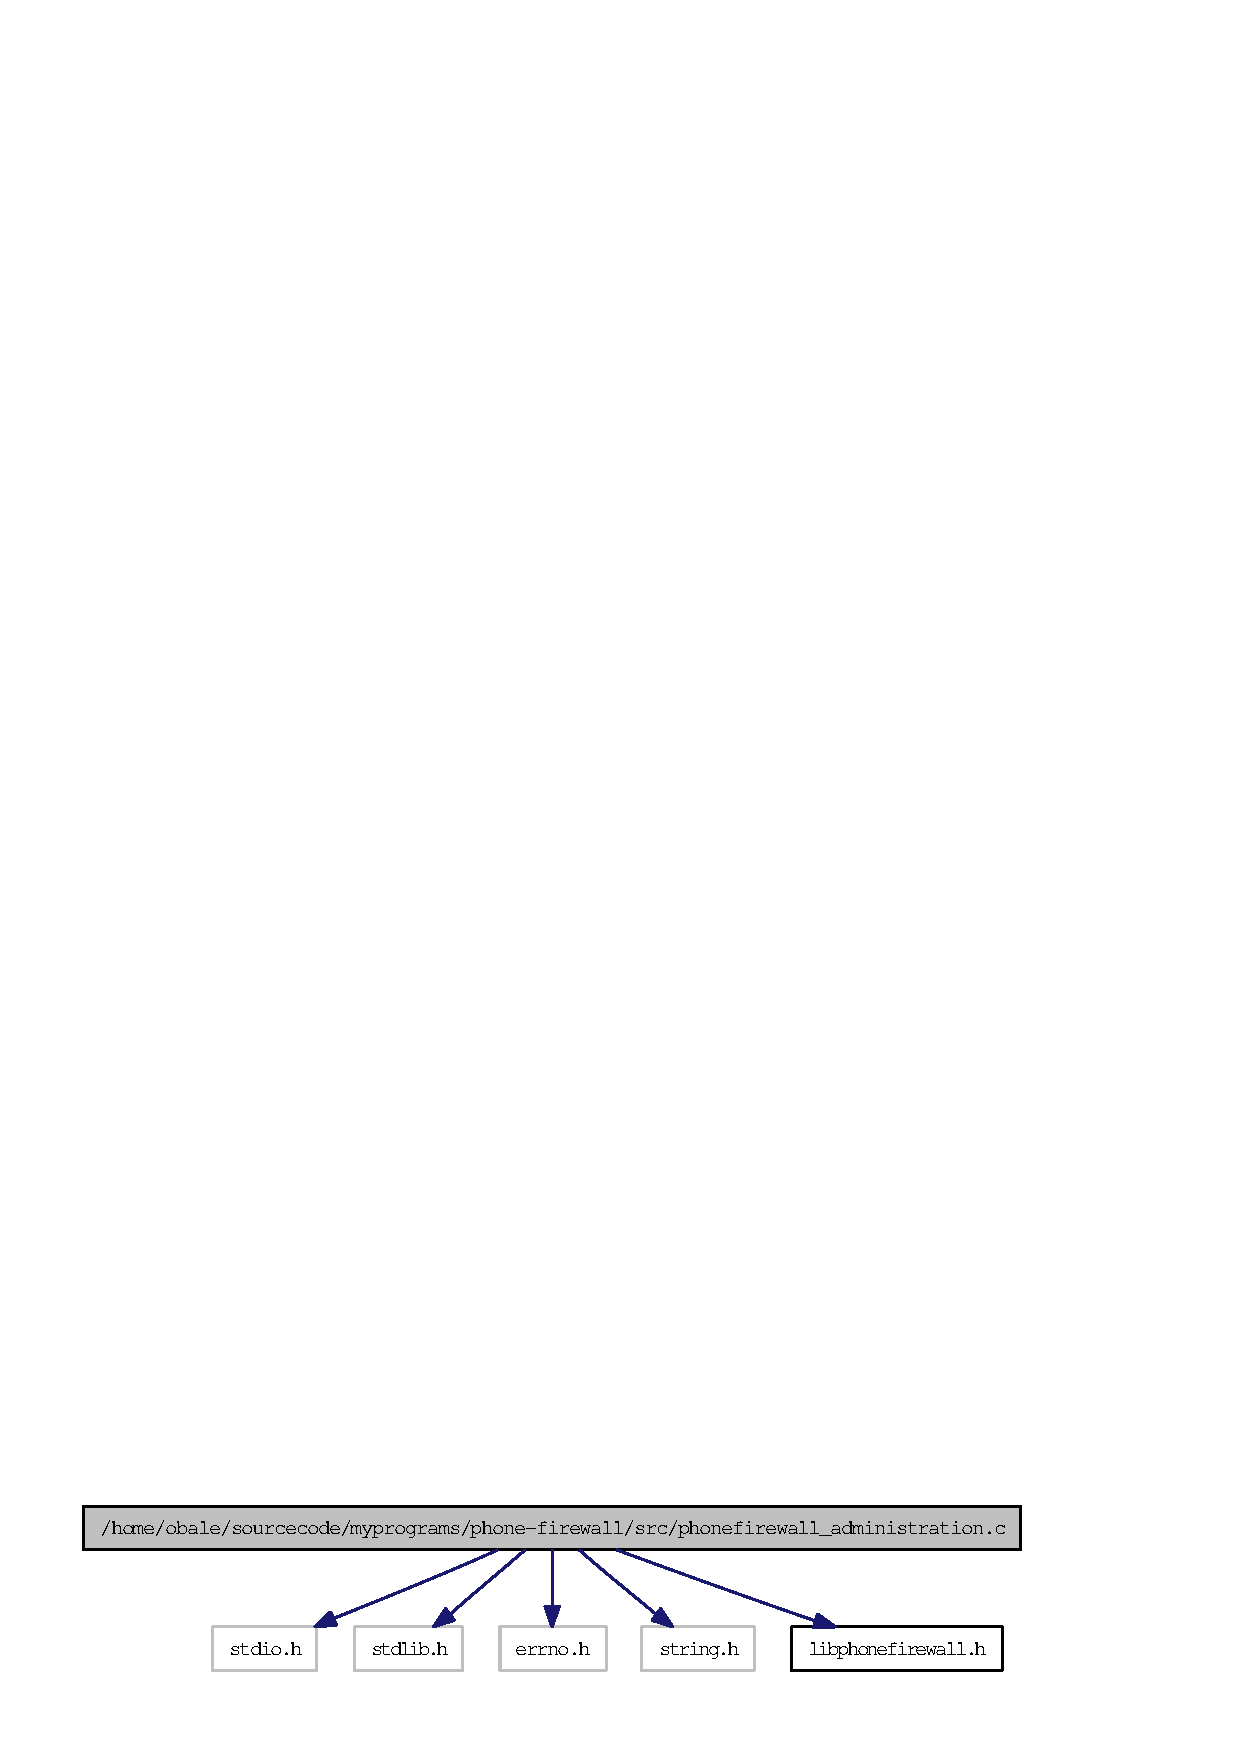
\includegraphics[width=247pt]{phonefirewall__administration_8c__incl}
\end{center}
\end{figure}
\subsection*{Functions}
\begin{CompactItemize}
\item 
int \hyperlink{phonefirewall__administration_8c_c779be47603de2c586393463c7c1cf40}{add\_\-blacklist\_\-entry} (char $\ast$number, char $\ast$name, char $\ast$reason, int priority)
\item 
int \hyperlink{phonefirewall__administration_8c_5054a65f2dffa39cd56ddbb852314e1a}{rm\_\-blacklist\_\-entry} (char $\ast$number)
\item 
int \hyperlink{phonefirewall__administration_8c_6ff23c996da4efd7ae26d38a317813e0}{add\_\-whitelist\_\-entry} (char $\ast$number, char $\ast$name, char $\ast$reason, int priority)
\item 
int \hyperlink{phonefirewall__administration_8c_be3e9ad52c2f2ab7fb9f9f30e37c2257}{rm\_\-whitelist\_\-entry} (char $\ast$number)
\end{CompactItemize}


\subsection{Function Documentation}
\hypertarget{phonefirewall__administration_8c_c779be47603de2c586393463c7c1cf40}{
\index{phonefirewall\_\-administration.c@{phonefirewall\_\-administration.c}!add\_\-blacklist\_\-entry@{add\_\-blacklist\_\-entry}}
\index{add\_\-blacklist\_\-entry@{add\_\-blacklist\_\-entry}!phonefirewall_administration.c@{phonefirewall\_\-administration.c}}
\subsubsection{\setlength{\rightskip}{0pt plus 5cm}int add\_\-blacklist\_\-entry (char $\ast$ {\em number}, char $\ast$ {\em name}, char $\ast$ {\em reason}, int {\em priority})}}
\label{phonefirewall__administration_8c_c779be47603de2c586393463c7c1cf40}


Add a number to the blacklist. The number will be blocked after that.

\begin{Desc}
\item[Parameters:]
\begin{description}
\item[{\em number}]The telephone number of the person. \item[{\em name}]The name of the person. \item[{\em reason}]Why you have blocked this person. \item[{\em priority}]Has no affect at the moment. Later one it will be possible to give each number priority. So you have more control when a number will be blocked/accepted.\end{description}
\end{Desc}
\begin{Desc}
\item[Returns:]If all goes well 0 (zero) otherwise an errno code. \end{Desc}


Definition at line 26 of file phonefirewall\_\-administration.c.

References MAX\_\-ENTRIES, Blacklist::name, Blacklist::number, Blacklist::reason, and TELNR\_\-MAXLEN.\hypertarget{phonefirewall__administration_8c_6ff23c996da4efd7ae26d38a317813e0}{
\index{phonefirewall\_\-administration.c@{phonefirewall\_\-administration.c}!add\_\-whitelist\_\-entry@{add\_\-whitelist\_\-entry}}
\index{add\_\-whitelist\_\-entry@{add\_\-whitelist\_\-entry}!phonefirewall_administration.c@{phonefirewall\_\-administration.c}}
\subsubsection{\setlength{\rightskip}{0pt plus 5cm}int add\_\-whitelist\_\-entry (char $\ast$ {\em number}, char $\ast$ {\em name}, char $\ast$ {\em reason}, int {\em priority})}}
\label{phonefirewall__administration_8c_6ff23c996da4efd7ae26d38a317813e0}


Add a number to the \hyperlink{structwhitelist}{whitelist}. The number will be accepted after that.

\begin{Desc}
\item[Parameters:]
\begin{description}
\item[{\em number}]The telephone number of the person. \item[{\em name}]The name of the person. \item[{\em reason}]Why you have blocked this person. \item[{\em priority}]Has no affect at the moment. Later one it will be possible to give each number priority. So you have more control when a number will be blocked/accepted.\end{description}
\end{Desc}
\begin{Desc}
\item[Returns:]If all goes well 0 (zero) otherwise an errno code. \end{Desc}


Definition at line 51 of file phonefirewall\_\-administration.c.\hypertarget{phonefirewall__administration_8c_5054a65f2dffa39cd56ddbb852314e1a}{
\index{phonefirewall\_\-administration.c@{phonefirewall\_\-administration.c}!rm\_\-blacklist\_\-entry@{rm\_\-blacklist\_\-entry}}
\index{rm\_\-blacklist\_\-entry@{rm\_\-blacklist\_\-entry}!phonefirewall_administration.c@{phonefirewall\_\-administration.c}}
\subsubsection{\setlength{\rightskip}{0pt plus 5cm}int rm\_\-blacklist\_\-entry (char $\ast$ {\em number})}}
\label{phonefirewall__administration_8c_5054a65f2dffa39cd56ddbb852314e1a}


Removes a blocked number from the blacklist. 

Definition at line 47 of file phonefirewall\_\-administration.c.\hypertarget{phonefirewall__administration_8c_be3e9ad52c2f2ab7fb9f9f30e37c2257}{
\index{phonefirewall\_\-administration.c@{phonefirewall\_\-administration.c}!rm\_\-whitelist\_\-entry@{rm\_\-whitelist\_\-entry}}
\index{rm\_\-whitelist\_\-entry@{rm\_\-whitelist\_\-entry}!phonefirewall_administration.c@{phonefirewall\_\-administration.c}}
\subsubsection{\setlength{\rightskip}{0pt plus 5cm}int rm\_\-whitelist\_\-entry (char $\ast$ {\em number})}}
\label{phonefirewall__administration_8c_be3e9ad52c2f2ab7fb9f9f30e37c2257}


Removes a accepted number from the \hyperlink{structwhitelist}{whitelist}. 

Definition at line 55 of file phonefirewall\_\-administration.c.